\documentclass[a4j,11pt]{jsarticle}
%jbbok:書籍・jsarticle:論文,短い文書・jreport:レポート・letter:手紙・twocolumn:2段組
\usepackage{amsmath,amsfonts,amssymb,mathtools,ascmac,bm,float,comment,url,fancybox,calc,subcaption,multicol,physics,tablefootnote,caption,graphics,multirow}
\usepackage{wrapfig}
\usepackage[T1]{fontenc}
\usepackage[margin=20truemm]{geometry}
\usepackage[dvipdfmx]{graphicx,color,hyperref}
\usepackage{tikz,listings,jlisting}
\usepackage{pxjahyper}
\usepackage{xcolor}
\hypersetup{
    colorlinks=true,
    citecolor=black,
    linkcolor=black,
    urlcolor=blue
}
        \tikzset{cy/.style={fill=cyan!10,rounded corners,rectangle,  text centered, minimum height=1cm}}
        \tikzset{ye/.style={fill=yellow!10,rounded corners,rectangle,  text centered, minimum height=1cm}}
        \tikzset{ma/.style={fill=magenta!10,rounded corners,rectangle,  text centered, minimum height=1cm,}}
        \tikzset{gr/.style={fill=green!10,rounded corners,rectangle,text centered,minimum height=1cm,text width=4.1cm}}
        \tikzset{Terminal/.style={rounded rectangle,  draw,  text centered, text width=3cm, minimum height=1.5cm}}
        \tikzset{Process/.style={rectangle,  draw,  text centered, text width=3cm, minimum height=1.5cm}}
        \tikzset{Decision/.style={diamond,  draw,  text centered, aspect=3,text width=5cm, minimum height=1.5cm}}
    \usetikzlibrary{arrows}
    \usetikzlibrary{intersections,calc,arrows.meta,backgrounds,shapes.geometric,shapes.misc,positioning,fit,graphs}
    \renewcommand{\lstlistingname}{src.}
    \newcommand{\srcref}[1]{src. \ref{#1}}
    \AtBeginDocument{
        % \renewcommand{\thelstlisting}{\thesection.\arabic{lstlisting}}
    }
    \lstset{
            %プログラム言語(複数の言語に対応,C,C++も可)
        language = Java,
            %背景色と透過度
        %backgroundcolor={\color[gray]{.90}},
            %枠外に行った時の自動改行
        breaklines = true,
            %自動改行後のインデント量(デフォルトでは20[pt])
        breakindent = 10pt,
            %標準の書体
        basicstyle = \ttfamily\small,
            %コメントの書体
        commentstyle = {\ttfamily \color[cmyk]{1,0.4,1,0}},
            %関数名等の色の設定
        classoffset = 0,
            %キーワード(int, ifなど)の書体
        keywordstyle = {\bfseries \color[cmyk]{0,1,0,0}},
            %表示する文字の書体
        stringstyle = {\ttfamily \color[rgb]{0,0,1}},
            %枠 tは上に線を記載, Tは上に二重線を記載
            %他オプション:leftline,topline,bottomline,lines,single,shadowbox
        frame = leftline,
            %frameまでの間隔(行番号とプログラムの間)
        framesep = 5pt,
            %行番号の位置
        % numbers = left,
            %行番号の間隔
        stepnumber = 1,
            %行番号の書体
        numberstyle = \small,
            %タブの大きさ
        tabsize = 4,
            %キャプションの場所(tbならば上下両方に記載)
        captionpos = t
    }
    \setlength{\columnsep}{5mm}
    \columnseprule=0.1mm
    \renewcommand{\thefootnote}{*\arabic{footnote}}
    \renewcommand{\figurename}{Fig\ }
    \renewcommand{\tablename}{Tbl\ }
    \newcommand{\figref}[1]{Fig\ \ref{#1}}
    \newcommand{\tabref}[1]{Tbl\ \ref{#1}}
    \newcommand{\met}[1]{\ttfamily #1 \normalfont (\srcref{src:#1})の処理}
\makeatletter
\renewcommand{\thefigure}{%
\arabic{figure}}
\@addtoreset{figure}{section}
\renewcommand{\thetable}{%
\arabic{table}}
\@addtoreset{table}{section}
% \@addtoreset{lstlisting}{section}
\makeatother
\renewcommand{\labelenumi}{\textbf{\arabic{enumi})\ }}


\title{\vspace{0cm}情報学群実験第1 最終レポート}
\author{1250373 溝口洸熙\thanks{高知工科大学 情報学群 2年生}}
\date{\today}


\begin{document}
%\twocolumn[
\maketitle
%]

\begin{abstract}
    このレポートは,情報学群実験第1の最終レポートである.
    マインスイーパーを作成し,それに対して指定された仕様1〜5と,追加した仕様6〜9の処理概要や処理の詳解がされている.仕様に対するソースコードは p.\pageref{sec:ソースコード}から記載している.
    実行は問題なくできており,仕様通りの動作となっている.この課題に取り組むに当たって,オブジェクト指向プログラミングの概念を再修得できた.
\end{abstract}
\newpage
\tableofcontents
\newpage
\section*{はじめに}
\addcontentsline{toc}{section}{はじめに}
\subsection*{レポートについて}
このレポートは,\LaTeXe を用いて作成している.図やグラフはTi\it{k}\normalfont Zを用いて描画しており,ソースコードはlistingを用いて表記している.
各参照には参照箇所まで誘導するリンクもついている.
\subsection*{符号化と変数}
あるパネルのステータスを示す符号と,新たに追加したグローバル変数を,以下に示す.
\begin{table}[h]
    \centering
    \begin{minipage}[t]{0.3\linewidth}
        \centering
        \subcaption*{符号とステータス}
        \label{tbl:符号とステータス}
        \begin{tabular}{cl}
            \hline
            符号 & \multicolumn{1}{c}{ステータス} \\
            \hline
            0    & 爆弾以外                       \\
            1    & 開かれたパネル                 \\
            -1   & 爆弾                           \\
            -2   & 旗が立っている                 \\
            \hline
        \end{tabular}
    \end{minipage}
    \begin{minipage}[t]{0.69\linewidth}
        \centering
        \subcaption*{新たに追加した変数}
        \begin{tabular}{ll}
            \hline
            \multicolumn{1}{c}{変数名} & \multicolumn{1}{c}{役割}                           \\
            \hline
            \verb|int originalTable|   & \begin{tabular}{l}
                                                  生成した盤面の初期状態を記憶する.
                                              \end{tabular}             \\
                                       &                                                    \\
            \verb|Boolean tr|          & \begin{tabular}{l}
                                                         2手目以降で\verb|true|になる変数. \\
                                                         1手目で爆弾に当たることを回避するため.
                                                     \end{tabular} \\
            \hline
        \end{tabular}
    \end{minipage}
\end{table}
また,このマインスイーパーはJavaのButtonクラスが使用されている.ボタンを離した時にアクションが起こるので,以下の情報を参考に,\verb|Main.java|を解読した.
\begin{screen}
    ボタンが押されて離されると、AWTはボタンのprocessEventを呼び出すことにより、ボタンにActionEventのインスタンスを送ります。ボタンのprocessEventメソッドはそのボタンのすべてのイベントを受け取ります。ボタンは自身のprocessActionEventメソッドを呼び出すことによってアクション・イベントを渡します。後者のメソッドはこのボタンによって生成されるアクション・イベントの通知を対象として登録されているアクション・リスナーにアクション・イベントを渡します。
    \cite{label1}
\end{screen}
\newpage
\part{必須仕様}
\section*{仕様1}
\setcounter{section}{1}
\addcontentsline{toc}{section}{仕様1}
\begin{screen}
    \textbf{仕様1.}\\
    ゲーム開始時に,盤面上へランダムに地雷を設置する.
\end{screen}
\subsection{処理概要}
\begin{figure}[h]
    \centering
    \caption{盤面上へランダムに地雷を設置する}
    \begin{tikzpicture}
        % \node[cy](initTable){\verb|void initTable()|};
        \node[Terminal](functionTable){\verb|initTable|};
        \node[Process,below=0.5cm of functionTable](functionMine){\verb|setMine|};
        \node[Decision,below=0.5cm of functionMine](checkBord){盤面を調査};
        \node[Process,below=0.5cm of checkBord](setNumber1){\verb|table|に\verb|0|を代入};
        \node[Process,below=0.5cm of setNumber1](setNumber2){\verb|originalTable|に\verb|0|を代入};
        \foreach \u \v in {functionTable/functionMine,functionMine/checkBord,setNumber1/setNumber2}
        \draw[-latex](\u)--(\v);
        \draw[-latex](checkBord)node[right,yshift=-40]{そのパネルが爆弾でなければ}--(setNumber1);

        \node[Terminal,right =3cm of functionTable](setMine){\verb|setMine|};
        \node[Process,below =0.5cm of setMine](set){\verb|numMine|の数だけ爆弾をセットする};

        \node[inner sep=0cm,fit={(setMine)(set)}](warp){};
        \node[inner sep=0cm,above=0.1cm of warp.north](caption){\verb|setMine|メソッド};
        \node[draw,dashed,rounded corners,fit={(warp)(caption)}](plate){};

        \foreach \u \v in {functionMine.east/plate,plate.west/functionMine}
        \draw[thick,-Stealth](\u)--(\v);
        \draw[-latex](setMine)--(set);
    \end{tikzpicture}
\end{figure}
\newpage
\subsection{処理}
\subsubsection*{\met{initTable}}
盤面を初期化するにあたって,以下の処理を行う.
\begin{enumerate}
    \item \verb|table,originalTable|の全ての行と列に\verb|0|を代入する.ただし,爆弾であるパネルは上書きしない.
    \item 爆弾の設置パネルを\verb|setMine|メソッドで定める.
          \begin{lstlisting}[caption=, label=, language=Java]
for (int i = 0; i < table.length; i++) {
    for (int j = 0; j < table.length; j++) {
        this.table[i][j] = 0;
        this.originalTable[i][j] = 0;
    }
}
this.setMine();
            \end{lstlisting}
\end{enumerate}
\subsubsection*{\met{setMine}}
盤面に爆弾を配置するにあたって,以下の処理を行う.
\begin{enumerate}
    \item 爆弾の個数を数える\verb|count|変数を定義する.
          \begin{lstlisting}[caption=, label=, language=Java]
int count = 0;
\end{lstlisting}
    \item 指定された爆弾の個数が\verb|count|になるまで,爆弾を配置する.
          \begin{lstlisting}[caption=, label=, language=Java]
while (count != this.numMine) {// numMineの数だけ爆弾をセットできたらループを抜ける
...
}
    \end{lstlisting}
    \item 爆弾の配置はランダムである.乱数で指定されたパネルが既に爆弾であれば再度乱数を生成し,爆弾が新たにセットできる場所では,\verb|table|,\verb|originalTable|の乱数値Indexを\verb|-1|に設定し,\verb|count|をインクリメントする.
          \begin{lstlisting}[caption=, label=, language=Java]
...
int x = new java.util.Random().nextInt(getHeight());
int y = new java.util.Random().nextInt(getWidth());
if (this.table[x][y] == -1) {
    // [x][y]にすでに爆弾がセットされていたら、もう一度乱数を決め直す
    continue;
}
count++;
...
    \end{lstlisting}
\end{enumerate}
\begin{flushright}
    \underline{仕様1 終}
\end{flushright}
\newpage
\section*{仕様2}
\setcounter{subsection}{0}
\addcontentsline{toc}{section}{仕様2}
\setcounter{section}{2}
\begin{screen}
    \textbf{処理2.}\\
    パネルを左クリックした際,クリックしたパネルを開く.
\end{screen}
\subsection{処理概要}
\begin{figure}[h]
    \centering
    \caption{タイルを開くときの処理}
    \begin{tikzpicture}
        \node[Terminal](openTile){\verb|openTile|};
        \node[Decision,below=0.4cm of openTile](turn){1手目で爆弾};
        \node[Decision,below=0cm of turn](flag){そのパネルに旗が立っている};
        \node[Terminal,right=1cm of flag](return2){\verb|return;|};
        \node[Decision,below=0cm of flag](mine){爆弾を踏んだ};
        \node[Process,fill=magenta!10,below=0.4cm of mine](quarityMine){周辺の爆弾の個数を数えて表示};
        \node[Process,fill=magenta!10,below=0.4cm of quarityMine](setNumber){開いたパネルを\verb|-1|に設定};
        \node[Decision,below=0.4cm of setNumber](serch){全てのパネルが開いたか};
        \node[Terminal,below=0.4cm of serch](win){\verb|gui.win()|の呼び出し};

        \node[Process,right=1cm of turn](setMine){\verb|initTable|};
        \node[Terminal,right=1cm of mine](lose){\verb|gui.lose()|の呼び出し};
        \node[Terminal,right=1cm of serch](return){\verb|return;|};

        \foreach \u \v in {openTile/turn,mine/quarityMine,quarityMine/setNumber,setNumber/serch,serch/win,turn/setMine,mine/lose,serch/return,flag/return2}
        \draw[-latex](\u)--(\v);
        \draw[-latex](setMine)|-(openTile);
        \foreach \x \z in {turn/No,flag/No,mine/No,serch/Yes}
        \node[right=0.5cm of \x.south]{\z};
        \foreach \x \z in {turn/Yes,mine/Yes,serch/No/,flag/No}
        \node[above=0cm of \x.east]{\z};

        \node[inner sep=0.05cm,fit={(quarityMine)(setNumber)}](warp){};
        \node[dashed,rounded corners,draw,fit={(warp)}](plate){};
        \node[inner sep=0cm,left=0.1cm of plate.north west](caption){\textbf{仕様2}};
    \end{tikzpicture}
\end{figure}
\newpage
\subsection{処理}\label{sec:openTile}
\subsubsection*{\met{openTile}の一部}
\begin{enumerate}
    \item パネルに爆弾がない場合,その周辺の爆弾個数を{\verb|returnMine|}(\srcref{src:returnMine})メソッドで取得し,そのパネルに表示する.
          \begin{lstlisting}[caption=, label=, language=Java]
String mc = String.valueOf(mineCount);
gui.setTextToTile(x, y, mc); // 爆弾の個数を表示
    \end{lstlisting}
    \item 全てのパネルが開いたか否か確認する.もし,全てのパネルが開いていたら勝利となるので{\verb|gui.win|}を呼び出し,開いていないパネルが存在すれば,{\verb|return;|}する.
          \begin{lstlisting}[caption=, label=, language=Java]
int mineCount = this.returnMine(x, y, gui);// 周辺の爆弾の個数を調査
this.table[x][y] = 1; // 開かれたパネルの値を1に設定
...
// 爆弾以外のパネルが全て開いているか確認
for (int i = 0; i < getHeight(); i++) {
    for (int j = 0; j < getWidth(); j++) {
        if (this.table[i][j] == 0) { return;}
    }
}
gui.win();
\end{lstlisting}
\end{enumerate}
\newpage

\section*{仕様3}
\setcounter{section}{3}
\addcontentsline{toc}{section}{仕様\thesection}
\setcounter{subsection}{0}
\begin{screen}
    \textbf{仕様\thesection.}\\
    開いたパネルに地雷が隠されている場合,全てのパネルを開く.
\end{screen}
\subsection{処理概要}
\begin{figure}[h]
    \centering
    \caption{全てのパネルを開く}
    \begin{tikzpicture}
        \node[Terminal](openTile){\verb|openTile|};
        \node[Process,below=0.5cm of openTile](otherProcess){その他の処理};
        \node[Decision,below=0.5cm of otherProcess](mine){爆弾を踏んだ};
        \node[Process,below=0.5cm of mine](specification2){仕様2,その他の処理};
        \node[Terminal,below=0.5cm of specification2](win){\verb|gui.win()|の呼び出し};

        \node[Terminal,right=4cm of openTile](openAllTiles){\verb|openAllTiles|};
        \node[Process,below=0.5cm of openAllTiles](decision1){様々な条件分岐};
        \node[Process,below=0.5cm of decision1](decision2){そのタイルが爆弾であれば,"\verb|B|"と表示};
        \node[Process,below=0.5cm of decision2](show){タイルの周りにある爆弾の数を表示};

        \node[inner sep=0.1cm,fit={(openAllTiles)(decision1)(decision2)(show)}](warp){};
        \node[dashed,rounded corners,draw,fit={(warp)}](plate){};

        \node[inner sep=0cm,fit={(decision1)}](warp_2){};
        \node[red,draw,rounded corners,dotted,thick,fit={(warp_2)}](plate_2){};
        \node[red,above left=-0.09cm of plate_2.north east]{\small 追加仕様};

        \foreach \u \v in {openTile/otherProcess,otherProcess/mine,mine/specification2,specification2/win,openAllTiles/decision1,decision2/show,decision1/decision2}
        \draw[-latex](\u)--(\v);
        \draw[Stealth-Stealth](mine.east)--(plate);
        \node[below=0.5cm of plate,Terminal](lose){\verb|gui.lose()|の呼び出し};
        \draw[-latex](plate)--(lose);
        \node[below right=0cm of mine.south]{No};
        \node[above=0.1cm of mine.east]{Yes};
    \end{tikzpicture}
\end{figure}
追加仕様に関しては,仕様8で詳説する.
\subsection{処理}\label{sec:仕様3処理}
全てのタイルに対して,条件分岐を行う.ただ単に全てのタイルに対して\verb|openTile|メソッドを呼び出してもよかったが,その仕様では,自分がどこにフラグを立てて,そのフラグが正しいか否かの判断ができかねる.
従って,\verb|openAllTiles|メソッド(\srcref{src:openAllTiles})に関しては,仕様8で詳解する.
\newpage

\section*{仕様4}
\addcontentsline{toc}{section}{仕様4}
\setcounter{section}{4}
\setcounter{subsection}{0}
\begin{screen}
    \textbf{仕様\thesection.}\\
    開いていないパネルを右クリックした際,そのパネルに旗を立てる.
    また,旗が立てられているパネルの場合には畑を取り除き,旗が取り除かれるまで左クリックでパネルは開けない.
\end{screen}
\subsection{処理の概要}
\begin{figure}[h]
    \centering
    \caption{旗を立てるときの処理}
    \begin{tikzpicture}
        \node[Terminal](setFlag){\verb|setFlag|};
        \node[Decision,below=0.5cm of setFlag](decision1){\small タイルが開かれていない\\かつ旗が立っていない};
        \node[Decision,below=0.5cm of decision1](decision2){旗が既に立っている};
        \node[Process,below=0.5cm of decision2](setF){タイルに旗を立てる};
        \node[Process,below=1cm of setF](delF){タイルから旗を除く};
        \node[Terminal,below=1cm of delF](return){\verb|return;|};

        \foreach \u \v in {setFlag/decision1,decision1/decision2,decision2/setF,setF/delF,delF/return}
        \draw[-latex](\u)--(\v);
        \foreach \u \v in {decision1/Yes,decision2/No}
        \node[below right=0cm of \u.south]{\v};
        \foreach \u \v in {decision1/No,decision2/Yes}
        \node[above right=0cm of \u.east]{\v};
        \node[right=3cm of return](return2){};
        \coordinate (A) at ($(decision1.east)$);
        \coordinate (B) at ($(decision2.east)$);
        \coordinate (C) at ($(decision1.east)+(1cm,0cm)$);
        \coordinate (D) at (C |- B);

        \draw(A)--(C)-|(D);
        \draw(B)--(D);
        \draw[-latex](D)|-(return.east);
    \end{tikzpicture}
\end{figure}
\newpage
\subsection{処理}
\subsubsection*{\met{setFlag}}
今,入力として\ \verb|x|行\verb|y|列\ のIndexが与えられた.
\begin{enumerate}
    \item そのタイルが開いていない時に旗を立てる.
          \begin{lstlisting}[caption=, label=, language=Java]
if (this.table[x][y] == 0 || this.table[x][y] == -1) {
    this.table[x][y] = -2; // 旗を立てる場所に-2を入れる
    gui.setTextToTile(x, y, "F");
}
    \end{lstlisting}
    \item そのタイルに既に旗が立っているとき,そのタイルを初期状態に戻す.
          \begin{lstlisting}[caption=, label=, language=Java]
else if (this.table[x][y] == -2) {
    this.table[x][y] = this.originalTable[x][y];
    gui.setTextToTile(x, y, "");
}
    \end{lstlisting}
\end{enumerate}
\dotfill
\begin{enumerate}
    \renewcommand{\labelenumi}{}
    \item \verb|openTile|メソッドで,タイルにはたがあるか,既に開けられたタイルであれば,\verb|return;|する処理がある.
          \begin{lstlisting}[caption=, label=, language=Java]
if (this.table[x][y] == 1 || this.table[x][y] == 2) {
    return;
}
        \end{lstlisting}
\end{enumerate}
\newpage
\section*{仕様5}
\setcounter{section}{5}
\addcontentsline{toc}{section}{仕様\thesection}
\setcounter{subsection}{0}
\begin{screen}
    \textbf{仕様\thesection.}\\
    クリアもしくはゲームオーバーになった際,適切なダイアログを表示する.
\end{screen}
\subsection{処理}
\begin{figure}[h]
    \centering
    \caption{ダイアログの表示}
    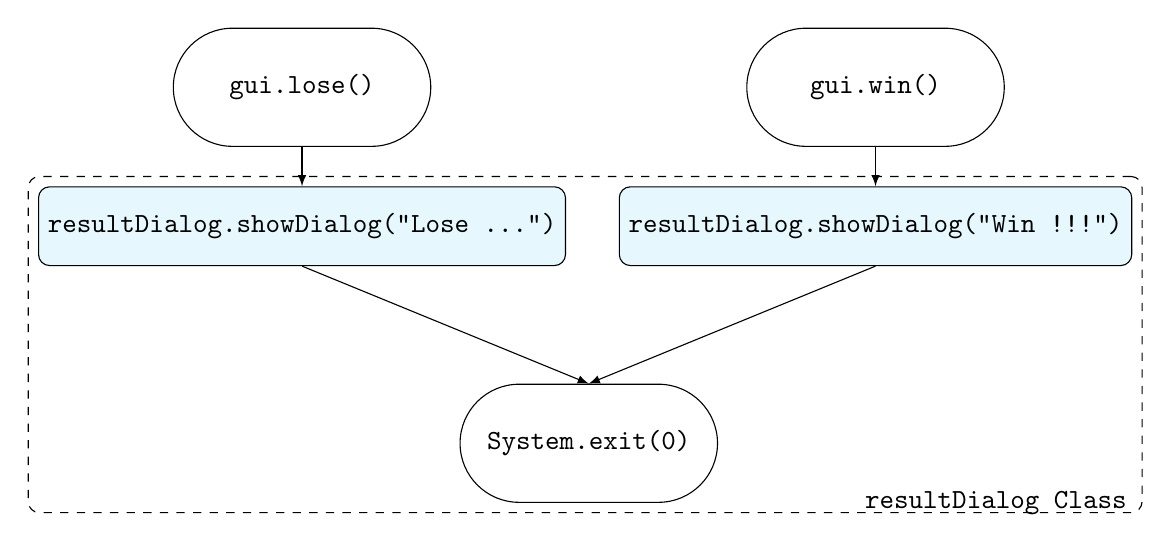
\begin{tikzpicture}[remember picture]
        \node[Terminal](lose){\verb|gui.lose()|};
        \node[Terminal,right=4cm of lose](win){\verb|gui.win()|};
        \node[draw,cy,below=0.5cm of win](dwin){\verb|resultDialog.showDialog("Win !!!")|};
        \node[draw,cy,below=0.5cm of lose](dlose){\verb|resultDialog.showDialog("Lose ...")|};
        \coordinate (A) at ($(dwin)!0.5!(dlose)$);
        \node[Terminal,below=2cm of A](exit){\verb|System.exit(0)|};

        \foreach \u \v in {win/dwin,lose/dlose,dwin/exit,dlose/exit}
        \draw[-latex](\u.south)--(\v.north);

        \node[inner sep=0cm,fit={(dwin)(dlose)(exit)}](warp){};
        \node[dashed,draw,rounded corners,fit={(warp)}](plate){};
        \node[right=2.5cm of exit.south east]{\verb|resultDialog Class|};
    \end{tikzpicture}
\end{figure}
\subsection{実装箇所}
\noindent\ovalbox{\verb|gui.lose|の実装箇所}\par
\verb|openTile|メソッド.爆弾を開けたとき.\\
\ovalbox{\verb|gui.win|の実装箇所}\par
\verb|openTile|メソッド.全てのタイルが開かれた,もしくは爆弾には旗が立っている場合.\\\par
Java仮想マシンを終了するには,\verb|System.exit(0)|の実行が必要.\verb|System.exit|に関しては以下を参照した.
\begin{screen}
    Systemクラスには有用なクラス・フィールドおよびメソッドがあります。インスタンス化することはできません。\\
    \verb|System.exit(int status)|\\
    現在実行しているJava仮想マシンを終了します。\cite{label2}
\end{screen}
\newpage
\part{追加仕様}
\section*{仕様6}
\setcounter{section}{6}
\addcontentsline{toc}{section}{仕様\thesection}
\setcounter{subsection}{0}
「運」のみで勝敗が決まるのは,ゲームとしては面白くない.プレイヤーは1手目から爆弾か否かを判断することは,不可能なので,1手目で爆弾のタイルを開けない仕様を追加した.
\subsubsection*{仕様6の実装}
\verb|openTile|メソッドにおいて,1手目で爆弾のタイルを選択した場合の条件分岐を設けている.
\begin{lstlisting}[caption=, label=, language=Java]
public void openTile(int x, int y, MineSweeperGUI gui) {
    ...
    if (this.table[x][y] == -1 && !this.tr) {
        this.initTable();
        this.openTile(x, y, gui);
    }
    this.tr=ture;
    ...
}
\end{lstlisting}
\section*{仕様7}
\setcounter{section}{7}
\setcounter{subsection}{0}
\addcontentsline{toc}{section}{仕様7}
実際のマインスイーパーは,数字ごとに色が決められている.今回作成したマインスイーパーも同様にタイルのテキストに色を設定するメソッドを作成した.(\srcref{src:setColorText})\par
さらに,爆弾のタイルや,既に開けているタイルを識別しやすくするため,タイルの背景色を変更するメソッドも作成した.(\srcref{src:setColorBackground})
以下を参考にして,\verb|Main.java|を変更した.
\begin{screen}
    このコンポーネントのバックグラウンド・カラーを設定します。バックグラウンド・カラーが各コンポーネントにそれぞれ異なる影響を与えます。\cite{label3}\\
    スタイルから取得できる型保証された色の列挙です。領域のフォアグラウンド用のColorTypeです。\cite{label4}
\end{screen}
\section*{仕様8}
\setcounter{section}{8}
\setcounter{subsection}{0}
\addcontentsline{toc}{section}{仕様8}
実際のマインスイーパーは,旗を立てたところが爆弾でなければ,旗にばつ印をつける使用になっている.また,旗の位置が正しければ,その旗は表示されたままだ.この機能を実装したいと思い,\verb|openAllTiles|メソッド(\srcref{src:openAllTiles})に幾らかの条件分岐を設けた.条件と表示の関係を\tabref{tbl:条件とタイルの色及び表示}に示す.
\begin{table}[h]
    \centering
    \caption{条件とタイルの色及び表示}
    \label{tbl:条件とタイルの色及び表示}
    \begin{tabular}{l|ccc}
        \hline
        \multicolumn{1}{c|}{\multirow{2}{*}{条件}} & \multicolumn{3}{c}{真の時の処理}                             \\
        \cline{2-4}
                                                   & 表示                             & 背景色   & 文字色         \\
        \hline
        爆弾の場所に旗が立っている                 & "\verb|F|"                       & 指定なし & 黒             \\
        爆弾でない場所に旗が立っている             & "\verb|XB|"                      & 黒       & 白             \\
        爆弾の場所に旗が立っていない               & "\verb|B|"                       & 赤       & black          \\
        周りの爆弾が0でかつ開けられていない        & ""                               & 白       & --             \\
        その他                                     & 周りの爆弾の個数                 & 指定なし & 個数に応じた色 \\
        \hline
    \end{tabular}
\end{table}
\newpage
\section*{仕様9}
\addcontentsline{toc}{section}{仕様9}
\setcounter{section}{9}
実際のマインスイーパーは,周辺にある爆弾の個数が0個の場合,\verb|0|と表示するのではない.周辺にある爆弾の数が0個の場合は,「その周辺のタイルを開けることができる」ということは,明らかであるため自動的に開けてくれるのだ.
今回作成したマインスイーパーでも,その機能を実装した.\par
\figref{fig:タイルの一部}に対して,\tikz{\node[rectangle,dotted,draw,minimum size=0.5cm,fill=cyan!10]{};}の色のタイルは,爆弾がないことを示している.これは明らかであり,プレーヤに無駄な労力をかけることになるので,プログラムで自動的に開けることにした.\par
\begin{figure}[h]
    \centering
    \caption{}
    \label{fig:タイルの一部}
    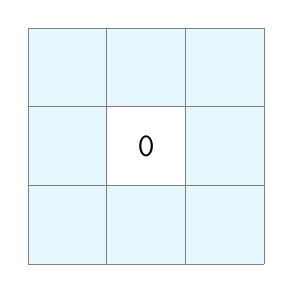
\begin{tikzpicture}[remember picture]
        \tikzset{gl/.style={rectangle,fill=cyan!10,minimum size=1cm}};
        \node at (1.5,1.5) (zero){\large\verb|0|};
        \foreach \u in {0.5,1.5,2.5}
        \node[gl]at(0.5,\u){};
        \foreach \u in {0.5,1.5,2.5}
        \node[gl]at(2.5,\u){};
        \node[gl]at(1.5,0.5){};
        \node[gl]at(1.5,2.5){};
        \draw[help lines, step=1cm](0,0) grid (3,3);
    \end{tikzpicture}
\end{figure}
範囲外を除いて,周りのタイルを再起的に開けていく方法をとった.これにより\tikz{\node[rectangle,dotted,draw,minimum size=0.5cm,fill=cyan!10]{};}の,タイルの周りの爆弾の個数が0個であったとしても,またさらにその周りのタイルを開けることができる.(これが再起の最大のメリットである.)
\begin{lstlisting}[caption=, label=, language=Java]
if (mineCount == 0) {// もし周辺に爆弾がなければ,そのマスも開ける.
for (int i = x - 1; i < x + 2; i++) {
    if (i < 0 || i >= getHeight()) { continue; }// 範囲外
    for (int j = y - 1; j < y + 2; j++) {
        if (j < 0 || j >= getWidth()) { continue; }// 範囲外
        openTile(i, j, gui);// 再起的に呼び出し
    }
}
\end{lstlisting}
\newpage
\part{ソースコード}\label{sec:ソースコード}
\noindent\ovalbox{\verb|MineSweeper.java > MineSweeper class|}
\lstset{frame=shadowbox,numbers=left}
\addcontentsline{toc}{section}{ソースコード}
\begin{lstlisting}[caption=\ttfamily initTable, label=src:initTable, language=Java]
void initTable() {
    for (int i = 0; i < table.length; i++) {
        for (int j = 0; j < table.length; j++) {
            this.table[i][j] = 0;
            this.originalTable[i][j] = 0;
        }
    }
    this.setMine();
}    
\end{lstlisting}
\begin{lstlisting}[caption=\ttfamily setMine, label=src:setMine, language=Java]
void setMine() {
    int count = 0;
    while (count != this.numMine) {// numMineの数だけ爆弾をセットできたらループを抜ける
        int x = new java.util.Random().nextInt(getHeight());
        int y = new java.util.Random().nextInt(getWidth());
        if (this.table[x][y] == -1) {
            // [x][y]にすでに爆弾がセットされていたら、もう一度乱数を決め直す
            continue;
        }
        this.table[x][y] = -1; // 爆弾の場所を値-1としてセットする
        this.originalTable[x][y] = -1;
        count++;
    }
}
\end{lstlisting}
\begin{lstlisting}[caption=\ttfamily openTile, label=src:openTile, language=Java]
public void openTile(int x, int y, MineSweeperGUI gui) {
	if (this.table[x][y] == 1 || this.table[x][y] == 2) {
		return;
	}
	if (this.table[x][y] == -1 && !this.tr) {// 1手目で爆弾ならば再度爆弾をセット
		this.initTable();
		this.openTile(x, y, gui);
	}
	this.tr = true;
	if (this.table[x][y] == -1) { // パネルに爆弾があった場合
		this.openAllTiles(gui);
		gui.lose();
	} else { // パネルに爆弾がなかった場合
		int mineCount = this.returnMine(x, y, gui);// 周辺の爆弾の個数を調査
		this.table[x][y] = 1; // 開かれたパネルの値を1に設定
		if (mineCount == 0) {// もし周辺に爆弾がなければ,そのマスも開ける
			for (int i = x - 1; i < x + 2; i++) {
				if (i < 0 || i >= getHeight()) { // パネルの範囲外は除く
					continue;
				}
				for (int j = y - 1; j < y + 2; j++) {
					if (j < 0 || j >= getWidth()) { // パネルの範囲外は除く
						continue;
					}
					openTile(i, j, gui);
				}
			}
		}
		String mc = String.valueOf(mineCount);
		if (mineCount == 0) {
			gui.setColorBackground(x, y, 0);
			gui.setTextToTile(x, y, "");
		} else {
			gui.setColorText(x, y, mineCount);// 色を設定
			gui.setTextToTile(x, y, mc); // 爆弾の個数を表示
		}
		for (int i = 0; i < getHeight(); i++) {// 爆弾以外のパネルが全て開いているか確認
			for (int j = 0; j < getWidth(); j++) {
				if (this.table[i][j] == 0) {
					return;
				}
			}
		}
		gui.win();
	}
}
\end{lstlisting}
\begin{lstlisting}[caption=\ttfamily returnMine, label=src:returnMine, language=Java]
private int returnMine(int x, int y, MineSweeperGUI gui) {
    int mineCount = 0;
    for (int i = x - 1; i < x + 2; i++) {
        if (i < 0 || i >= getHeight()) { // パネルの範囲外は除く
            continue;
        }
        for (int j = y - 1; j < y + 2; j++) {
            if (j < 0 || j >= getWidth()) { // パネルの範囲外は除く
                continue;
            }
            if (this.originalTable[i][j] == -1) { // 爆弾の個数をカウント
                mineCount++;
            }
        }
    }
    return mineCount;
}
\end{lstlisting}
\begin{lstlisting}[caption=\ttfamily openAllTiles, label=src:openAllTiles, language=Java]
private void openAllTiles(MineSweeperGUI gui) {
    for (int x = 0; x < getHeight(); x++) {
        for (int y = 0; y < getWidth(); y++) {
            Integer i = this.returnMine(x, y, gui);
            if (this.originalTable[x][y] == -1 && this.table[x][y] == -2) {// 爆弾の場所にフラグ
                gui.setTextToTile(x, y, "F");
                this.table[x][y] = 1;
            } else if (this.originalTable[x][y] != -1 && this.table[x][y] == -2) {// 爆弾でない場所にフラグ
                gui.setTextToTile(x, y, "XB");
                gui.setColorBackground(x, y, 3);
                gui.setColorText(x, y, 0);
            } else if (this.originalTable[x][y] == -1 && this.table[x][y] != 1) {// 爆弾の場所にフラグがない
                gui.setColorBackground(x, y, 2);
                gui.setColorText(x, y, 4);
                gui.setTextToTile(x, y, "B");
            } else if (i == 0 && this.table[x][y] != 1) {// 開けられていない場所の周りの爆弾の個数が0
                gui.setColorBackground(x, y, 0);
                gui.setTextToTile(x, y, "");
            } else {
                gui.setColorText(x, y, i);
                gui.setTextToTile(x, y, i.toString());
            }
        }
    }
}
\end{lstlisting}
\begin{lstlisting}[caption=\ttfamily setFlag, label=src:setFlag, language=Java]
public void setFlag(int x, int y, MineSweeperGUI gui) {
    if (this.table[x][y] == 0 || this.table[x][y] == -1) {
        this.table[x][y] = -2; // 旗を立てる場所に-2を入れる
        gui.setTextToTile(x, y, "F");
    } else if (this.table[x][y] == -2) {
        // すでに旗が立っているときは元の盤面の値に戻す
        this.table[x][y] = this.originalTable[x][y];
        gui.setTextToTile(x, y, "");
    }
}
\end{lstlisting}
\newpage
\ovalbox{\verb|Main.java > Main class|}
\begin{lstlisting}[caption=\ttfamily setColorText, label=src:setColorText,language=Java]
@Override
public void setColorText(int x, int y, int num) {
    switch (num) {
        case 1:
            this.tileTable[y][x].setForeground(Color.blue);
            break;
        case 2:
            this.tileTable[y][x].setForeground(new Color(0, 125, 0));
            break;
        case 3:
            this.tileTable[y][x].setForeground(Color.red);
            break;
        case 4:
            this.tileTable[y][x].setForeground(new Color(0, 0, 97));
            break;
        case 0:
            this.tileTable[y][x].setForeground(Color.white);
            break;
        default:
            this.tileTable[y][x].setForeground(Color.black);
    }
}
\end{lstlisting}
\begin{lstlisting}[caption=\ttfamily setColorBackground, label=src:setColorBackground,language=Java]
public void setColorBackground(int x, int y, int color) {
    switch (color) {
        case 0:
            this.tileTable[y][x].setBackground(Color.white);
            break;
        case 1:
            this.tileTable[y][x].setBackground(new Color(200, 255, 255));// new Color(RGB)
            break;
        case 2:
            this.tileTable[y][x].setBackground(Color.red);// new Color(RGB)
            break;
        case 3:
            this.tileTable[y][x].setBackground(Color.black);
            break;
    }
}
\end{lstlisting}
\part{まとめ}
今回のマインスイーパーの課題を通して,様々な学びがあった.\par
ゲームを模範して作るとなると,そのゲームのルールや性質をしっかりと学ぶ必要がある.幸にして,私は小学生の頃からマインスイーパーに触れており,(Windows xp内蔵)ルールの理解という面では苦労しなかった.\par
しかし,実際にアルゴリズムとしてマインスイーパーを考えると,なかなか簡単にはいかず,一つ一つの処理を詳細に,かつ順を追って見ていく必要があった.コンピュータは正直者なので,少しでも違う条件を与えると,当然だが予想だにしない挙動をする.
これがプログラミングの面白いところであるが,同時に難点でもある.一つ一つの処理が何を指すのか,その処理が無駄ではないのかなどを熟考した期間はとても充実していた.\par
今回作成したマインスイーパーにはまだ課題もある.それは,やや処理効率がわるいということだ.今回の課題では,それほど大きな2次元配列を扱うことはなかったが,これが大きな2次元配列になると,二重ループは好ましくない.(\(O(n^2)\)の時間がかかる故.)従って,今後は別の配列に対して,今の情報を格納する方法も検討したい.
メモリーの問題も生じると思うので,実験の結果を見て,より良い解決策を模索したい.\par
最後に,このレポートをここまで読んでくださった指導者の方に感謝申し上げる.
\begin{thebibliography}{99}
    \bibitem{label1} Java(tm) Platform Standard Edition 8 クラスButton(\today 最終確認)\\
    \url{https://docs.oracle.com/javase/jp/8/docs/api/java/awt/Button.html}
    \bibitem{label2} Java(tm) Platform Standard Edition 8 クラスSystem(\today 最終確認)\\
    \url{https://docs.oracle.com/javase/jp/8/docs/api/java/lang/System.html}
    \bibitem{label3} Java(tm) Platform Standard Edition 8 クラスComponent(\today 最終確認)\\
    \url{https://docs.oracle.com/javase/jp/8/docs/api/java/awt/Component.html}
    \bibitem{label4} Java(tm) Platform Standard Edition 8 クラスColorType(\today 最終確認)\\
    \small\url{https://docs.oracle.com/javase/jp/8/docs/api/javax/swing/plaf/synth/ColorType.html}
\end{thebibliography}

\end{document}